\documentclass[]{article}

%opening
\title{Notes/Phase I: Enumeration}
\author{Stefan O. Gugler}


\usepackage{graphicx} % Allows including images
\usepackage{booktabs} % Allows the use of \toprule, \midrule and \bottomrule in tables
\usepackage{pdfpages}
\usepackage[percent]{overpic}

\usepackage{tikz}
\usetikzlibrary{calc,trees,positioning,arrows,chains,shapes.geometric,%
	decorations.pathreplacing,decorations.pathmorphing,shapes,%
	matrix,shapes.symbols}

\tikzset{
	>=stealth',
	punktchain/.style={
		rectangle, 
		rounded corners, 
		% fill=black!10,
		draw=black, very thick,
		text width=10em, 
		minimum height=3em, 
		text centered, 
		on chain},
	line/.style={draw, thick, <-},
	element/.style={
		tape,
		top color=white,
		bottom color=blue!50!black!60!,
		minimum width=8em,
		draw=blue!40!black!90, very thick,
		text width=10em, 
		minimum height=3.5em, 
		text centered, 
		on chain},
	every join/.style={->, thick,shorten >=1pt},
	decoration={brace},
	tuborg/.style={decorate},
	tubnode/.style={midway, right=2pt},
}

\newcommand*\circled[1]{\tikz[baseline=(char.base)]{
		\node[shape=circle,draw,inner sep=2pt] (char) {#1};}}
	
%% Setting box counter
\newcounter{infobox}[section]
\renewcommand{\theinfobox}{\thesection.\arabic{infobox}}
 
\usepackage[framemethod=TikZ]{mdframed}
 
%% Infobox style
\newenvironment{infobox}[1][]{%
    \refstepcounter{infobox}
    \begin{mdframed}[%
        frametitle={Box \theinfobox\ #1},
        skipabove=\baselineskip plus 2pt minus 1pt,
        skipbelow=\baselineskip plus 2pt minus 1pt,
        frametitleaboveskip= 7pt,
        frametitlebelowskip= 7pt,
        linewidth=0pt,
        linecolor=black,
        frametitlerule=false,
        frametitlebackgroundcolor=blue!10,
        backgroundcolor=blue!10,
        roundcorner=7pt,
    ]%
}{%
    \end{mdframed}
}	
		
\begin{document}

\maketitle

\begin{abstract}
ACS Boston Abstract: Enumerating the inorganic universe of small complexes for machine learning. Transition metal complexes form promising functional inorganic materials due to their wide range of tunable electronic properties. However, exhaustive enumeration and calculation of all possible ligand fields is clearly intractable due to the vast nature of chemical space. Virtual high-throughput screening with density functional theory (DFT) allows us to harvest leads with desired properties but is severely constrained by 1) long calculation times and 2) variable accuracy. More accurate correlated methods are available to address 2) but drastically worsen 1). Machine learning techniques potentially allow us to address both issues simultaneously. Our group has previously developed data-driven models based on DFT results which have highlighted the dominant role of metal-proximal atoms (i.e. from the first and second coordination shell) in predicting spin state ordering, bond lengths, and ionization potential of the metal center. This motivates a systematic exploration of the space of octahedral complexes made of organic ligands with up to two heavy atoms (CNOPS), representing the metal-proximal environment. Even in this limited space, the number of potential candidate complexes is infeasible to calculate and so we propose a family of scoring functions that are used to extract mono- and bidentate ligands that most likely form stable complexes based on valency, net charge, and steric effects. The resulting organic ligand universe is then compared to similar studies of small organic molecules. Exploiting isoelectronic structure and empirical stability learned from previous studies, we sample the most promising compounds from this space with high-throughput DFT. We assess DFT performance selectively with more accurate correlated wavefunction calculations using domain-based local pair-natural orbital coupled cluster (DLPNO-CCSD(T)) and apply machine learning to model the difference between correlated wavefunction and DFT results in a composition-dependent manner. By doing this, we hope to learn property estimates for the full space of possible metal-proximal environments along with estimates of DFT reliability relative to DLPNO-CCSD(T).
\end{abstract}

\section{Enumeration}
\subsection{Introduction and Specifications}
Even though our chemical space is truncated to the first and second coordination shell, which allows us to use a maximum of two heavy atoms, $e \in \{C,N,O,P,S\} $ per ligand, it is still enormously big. In a first step we assemble the ligands and in a second step we attach them combinatorially to a metal center to produce octahedral complexes. 

For the ligand design, a number of parameters are introduced to later impose constraints on them to further decrease the vastness of the space. These parameters include the number of H atoms bond to any atom, $h^i_j$, the charge $c^i_j$, the number of lone pairs $l^i_j$, the number of valence electrons $v^i_j$, where $i$ and $j$ are the ligand's denticity and the atom index inside the ligand, respectively. We only build mono-heavy-atomic ligands (MHALs), di-heavy-atomic ligands (DHALs), and bidentate tetra-heavy-atomic ligands (THALs), which are two identical DHALs bonded together, imposing a strong symmetry constraint.

The full combinatorial space is first reduced via heuristics from classical chemistry like charge, sterics, satisfaction of the octet rule, whether the ligand is open or closed shell and bond orders. The most unfeasible candidates are not even scored all others are scored according to the heuristics mentioned above. The next reduction step is a cutoff over a certain score to obtain a space of desired and sensible structures, yet still too large to even enumerate, let alone calculate. To obtain a feasible space to enumerate, we sample a certain percentage from the the desired space weighted over the distribution of isoelectronic stuctures. This space is small enough to be enumerated. Samples are drawn randomly (?) to obtain DFT results and to interpolate the rest of the enumerated space (see Figure \ref{fig:truncation}).
 
 \begin{figure}[]
 \centering
 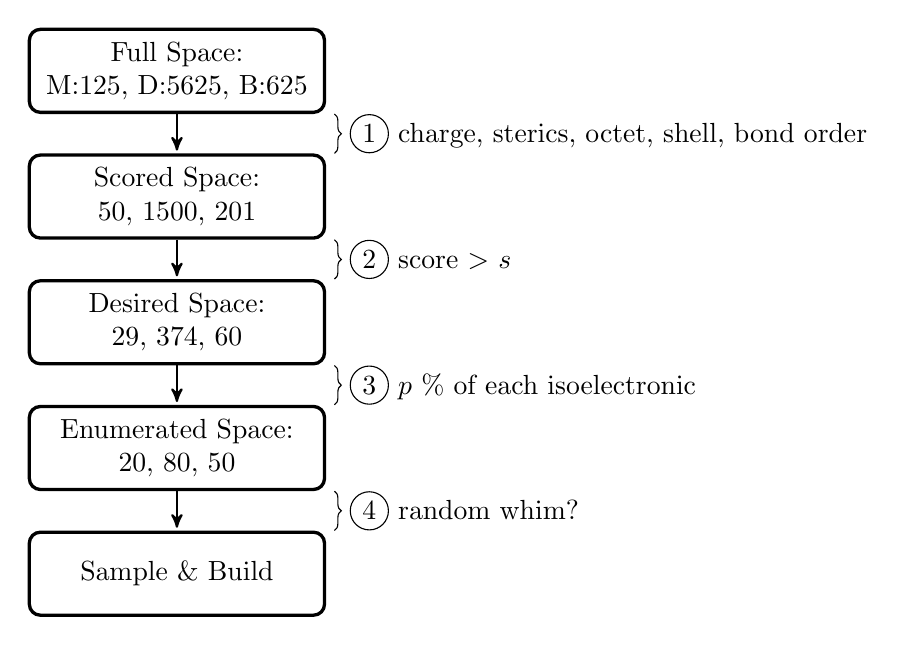
\begin{tikzpicture}
 [node distance=.5cm,
 start chain=going below,]
 \node[punktchain, join] (full) {Full Space: \\ M:125, D:5625, B:625};
 \node[punktchain, join] (scored){Scored Space: \\ 50, 1500, 201};
 \node[punktchain, join] (desi){Desired Space: \\ 29, 374, 60};
 \node[punktchain, join] (enum){Enumerated Space: \\ 20, 80, 50};
 \node[punktchain, join] (sampl){Sample \& Build };
 
 \draw[tuborg, decoration={brace}] let \p1=(full.south), \p2=(scored.north) in
 ($(2, \y1)$) -- ($(2, \y2)$) node[tubnode] {\circled{1} charge, sterics, octet, shell, bond order};
 \draw[tuborg] let \p1=(scored.south), \p2=(desi.north) in
 ($(2, \y1)$) -- ($(2, \y2)$) node[tubnode] {\circled{2} score $>$ $s$};
 \draw[tuborg] let \p1=(desi.south), \p2=(enum.north) in
 ($(2, \y1)$) -- ($(2, \y2)$) node[tubnode] {\circled{3} $p$ \% of each isoelectronic};
 \draw[tuborg] let \p1=(enum.south), \p2=(sampl.north) in
 ($(2, \y1)$) -- ($(2, \y2)$) node[tubnode] {\circled{4} random whim?};
 \end{tikzpicture}
 \caption{A diagram delineating the steps taken to truncate the full space into a space feasible for enumeration. The three numbers under the space label denote the number of mono-heavy-atomic, di-heavy-atomic, and tetra-heavy-atomic bidentate ligands obtained after the reduction step. On the right, the reduction criteria are listed.}
 \label{fig:truncation}
 \end{figure}
 
 \begin{infobox}[Valency (IUPAC Definition)]
 The maximum number of univalent atoms (originally hydrogen or chlorine atoms) that may combine with an atom of the element under consideration, or with a fragment, or for which an atom of this element can be substituted.
 \label{info:valency}
 \end{infobox}
 
\subsection{Spanning the full space}
For each element CNOPS we allow a charge $c \in \{-2,-1,0,1,2\}$ (we suppress the denticity and atom indices $i$ and $j$ where it is clear from the context) and a number of attached hydrogen atoms $h \in \{0,1,2,3,4\}$.

For the \textbf{MHALs}, we combinatorially cycle through all combinations of elements, of charge, and of number of H atoms, resulting in $5^3=125$ candidates. 

The \textbf{DHALs} were enumerated similarly, iterating through $e_1$, $e_2$, $h_1$, and $h_2$. Since, from a DFT perspective, charge is not a local property, we don't iterate over all combinations of $c_1$ and $c_2$, since it would produce many degeneracies (i.e. $-1+1=0$ is the same overall charge as $-2+2=0$) and it would not be clear, which charge distribution would be the right one, from a classical picture. For that reason, we iterate over a total charge $c_{tot}$. For every instance of $c_{tot}$, we call a subroutine that exhaustively checks all charge combinations that could result in $c_{tot}$. For each combination of charges $c_1$ and $c_2$, we calculate the valency $\nu$ (see Box \ref{info:valency}) of the respective atom as follows, given the lone pairs, $l_i$ and valence electrons $v_i$ from previous knowledge:

\begin{equation}
\label{eq:valency}
\nu_i = v_i - c_i - 2 \cdot l_i - 2 \cdot h_i ~. 
\end{equation}

We set the bond order $b$ to be the minimum of the valencies of the two atoms in the DHAL,
\begin{equation}
b = \min{\{\nu_1,\nu_2\}} ~,
\end{equation}
if the absolute difference of $\nu_1$ and $\nu_2$ is smallest over all charge combinations and $0 \leq b \leq 4$. The optimal charge distribution over the two atoms is assumed to be the $c_1$ and $c_2$ fulfilling the requirements above.

Since the \textbf{THALs} are composed of two bonded DHALs (labeled 1 and 2 for the first DHAL and $1^\prime$ and $2^\prime$ for the second DHAL, 1 and $1^\prime$ being the connecting atom), instead of building them from scratch, we decided to combine all the DHALs and exclude the ones that do not bond effectively. As before, we iterate through $e_1$, $e_2$, $h_1$, and $h_2$ of the building block DHAL. Similarly as with the regular DHAL enumeration described above, we assign a total charge $c_{tot}$ to one of the building block DHALs. We cycle then through all combinations of $c_1$ and $c_2$ and calculate the valencies of each atom according to Eq. (\ref{eq:valency}). If $\nu_1 > 0$, it means that it has at least one electron to bond with atom 2 and if $\nu_2 > 1$, it means that it has at least two electrons, one to bond with atom 1 and one to bond with atom $2^\prime$ of the other DHAL. Since the problem is symmetrical, the valencies $\nu_{1^\prime} > 0$ and $\nu_{2^\prime} > 0$ are exactly the same and only labeled differently to speak about them more effectively. The bond order $b_{12} \in \{1, ..., \nu_2\}$ is chosen as
\begin{equation}
\min_b\{|\nu_2 - \nu_2 - b_{12}|\}
\end{equation}
from which we can simply calculate the second bond, $b_{23}$, as
\begin{equation}
b_{23} = \min\{\nu_1, \nu_2 - b_{12}\} ~.
\end{equation}
We have two possibilities to choose the best charge and bond distribution: Either we require to have minimal bond orders or minimal absolute charges. We decided in favor of minimal charges, since this promises better stability for the resulting complexes. So, if $|c_1|$ and $|c_2|$ are smallest, we choose the corresponding bond orders and charges as the best ones.

\centering
\begin{overpic}[width=0.8\linewidth]{../meetings/18-03-28-flashtalk/img/distrDiCNOPS.pdf}
	\put (13,24) {[C--]=[OH2--]}
	\put (15,31) {[N--]-[PH4--]}
	\put (25,37) {[CH3]-[SH2-]}
	\put (30,45) {[PH++]\#0[SH3-]}
	
	\put (56,53) {[NH2]-[OH]}
	\put (80,57) {[C+]\#[O-]}
	\put (78,51) {[O-]\#[O-]}
\end{overpic}

\end{document}
